% Created by tikzDevice version 0.12 on 2019-07-24 05:12:26
% !TEX encoding = UTF-8 Unicode
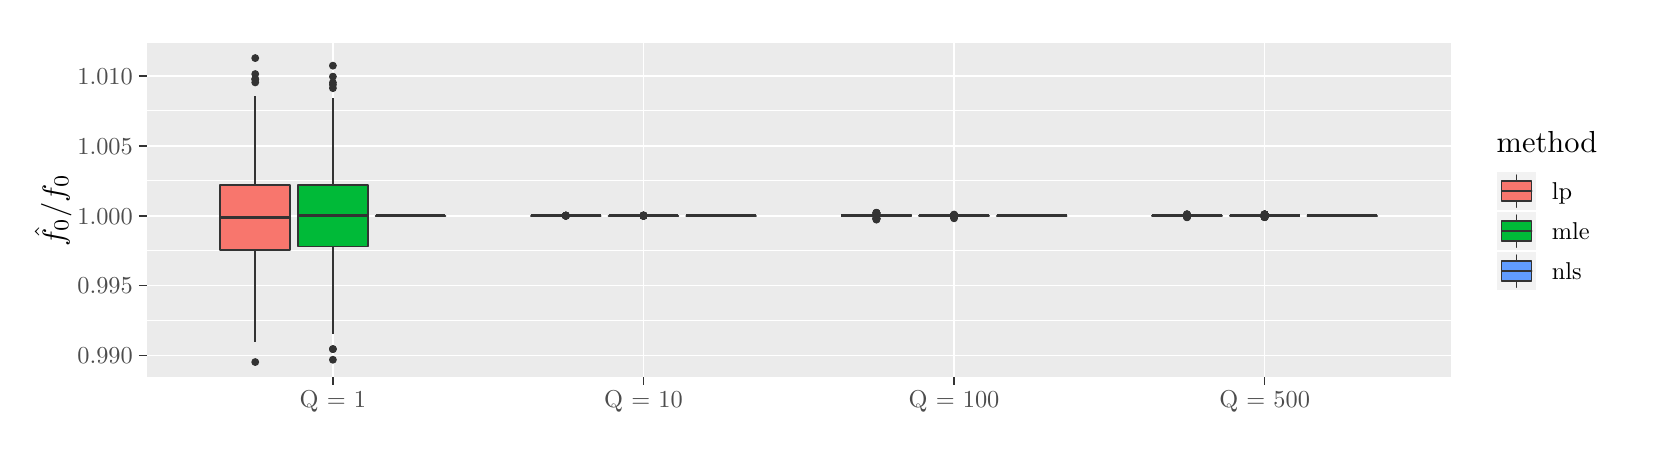
\begin{tikzpicture}[x=1pt,y=1pt]
\definecolor{fillColor}{RGB}{255,255,255}
\path[use as bounding box,fill=fillColor,fill opacity=0.00] (0,0) rectangle (578.16,144.54);
\begin{scope}
\path[clip] (  0.00,  0.00) rectangle (578.16,144.54);
\definecolor{drawColor}{RGB}{255,255,255}
\definecolor{fillColor}{RGB}{255,255,255}

\path[draw=drawColor,line width= 0.6pt,line join=round,line cap=round,fill=fillColor] (  0.00,  0.00) rectangle (578.16,144.54);
\end{scope}
\begin{scope}
\path[clip] ( 42.95, 18.22) rectangle (514.31,139.04);
\definecolor{fillColor}{gray}{0.92}

\path[fill=fillColor] ( 42.95, 18.22) rectangle (514.31,139.04);
\definecolor{drawColor}{RGB}{255,255,255}

\path[draw=drawColor,line width= 0.3pt,line join=round] ( 42.95, 38.73) --
	(514.31, 38.73);

\path[draw=drawColor,line width= 0.3pt,line join=round] ( 42.95, 63.98) --
	(514.31, 63.98);

\path[draw=drawColor,line width= 0.3pt,line join=round] ( 42.95, 89.23) --
	(514.31, 89.23);

\path[draw=drawColor,line width= 0.3pt,line join=round] ( 42.95,114.48) --
	(514.31,114.48);

\path[draw=drawColor,line width= 0.6pt,line join=round] ( 42.95, 26.10) --
	(514.31, 26.10);

\path[draw=drawColor,line width= 0.6pt,line join=round] ( 42.95, 51.35) --
	(514.31, 51.35);

\path[draw=drawColor,line width= 0.6pt,line join=round] ( 42.95, 76.60) --
	(514.31, 76.60);

\path[draw=drawColor,line width= 0.6pt,line join=round] ( 42.95,101.85) --
	(514.31,101.85);

\path[draw=drawColor,line width= 0.6pt,line join=round] ( 42.95,127.11) --
	(514.31,127.11);

\path[draw=drawColor,line width= 0.6pt,line join=round] (110.29, 18.22) --
	(110.29,139.04);

\path[draw=drawColor,line width= 0.6pt,line join=round] (222.52, 18.22) --
	(222.52,139.04);

\path[draw=drawColor,line width= 0.6pt,line join=round] (334.74, 18.22) --
	(334.74,139.04);

\path[draw=drawColor,line width= 0.6pt,line join=round] (446.97, 18.22) --
	(446.97,139.04);
\definecolor{drawColor}{gray}{0.20}
\definecolor{fillColor}{gray}{0.20}

\path[draw=drawColor,line width= 0.4pt,line join=round,line cap=round,fill=fillColor] ( 82.23,127.78) circle (  1.21);

\path[draw=drawColor,line width= 0.4pt,line join=round,line cap=round,fill=fillColor] ( 82.23,133.55) circle (  1.21);

\path[draw=drawColor,line width= 0.4pt,line join=round,line cap=round,fill=fillColor] ( 82.23,125.91) circle (  1.21);

\path[draw=drawColor,line width= 0.4pt,line join=round,line cap=round,fill=fillColor] ( 82.23,124.76) circle (  1.21);

\path[draw=drawColor,line width= 0.4pt,line join=round,line cap=round,fill=fillColor] ( 82.23,125.97) circle (  1.21);

\path[draw=drawColor,line width= 0.4pt,line join=round,line cap=round,fill=fillColor] ( 82.23, 23.71) circle (  1.21);

\path[draw=drawColor,line width= 0.6pt,line join=round] ( 82.23, 87.69) -- ( 82.23,119.96);

\path[draw=drawColor,line width= 0.6pt,line join=round] ( 82.23, 64.28) -- ( 82.23, 31.04);
\definecolor{fillColor}{RGB}{248,118,109}

\path[draw=drawColor,line width= 0.6pt,line join=round,line cap=round,fill=fillColor] ( 69.61, 87.69) --
	( 69.61, 64.28) --
	( 94.86, 64.28) --
	( 94.86, 87.69) --
	( 69.61, 87.69) --
	cycle;

\path[draw=drawColor,line width= 1.1pt,line join=round] ( 69.61, 75.87) -- ( 94.86, 75.87);
\definecolor{fillColor}{gray}{0.20}

\path[draw=drawColor,line width= 0.4pt,line join=round,line cap=round,fill=fillColor] (110.29,124.69) circle (  1.21);

\path[draw=drawColor,line width= 0.4pt,line join=round,line cap=round,fill=fillColor] (110.29,126.85) circle (  1.21);

\path[draw=drawColor,line width= 0.4pt,line join=round,line cap=round,fill=fillColor] (110.29, 28.41) circle (  1.21);

\path[draw=drawColor,line width= 0.4pt,line join=round,line cap=round,fill=fillColor] (110.29,123.91) circle (  1.21);

\path[draw=drawColor,line width= 0.4pt,line join=round,line cap=round,fill=fillColor] (110.29,130.81) circle (  1.21);

\path[draw=drawColor,line width= 0.4pt,line join=round,line cap=round,fill=fillColor] (110.29, 28.38) circle (  1.21);

\path[draw=drawColor,line width= 0.4pt,line join=round,line cap=round,fill=fillColor] (110.29,122.68) circle (  1.21);

\path[draw=drawColor,line width= 0.4pt,line join=round,line cap=round,fill=fillColor] (110.29, 24.54) circle (  1.21);

\path[draw=drawColor,line width= 0.6pt,line join=round] (110.29, 87.62) -- (110.29,119.26);

\path[draw=drawColor,line width= 0.6pt,line join=round] (110.29, 65.42) -- (110.29, 33.88);
\definecolor{fillColor}{RGB}{0,186,56}

\path[draw=drawColor,line width= 0.6pt,line join=round,line cap=round,fill=fillColor] ( 97.66, 87.62) --
	( 97.66, 65.42) --
	(122.92, 65.42) --
	(122.92, 87.62) --
	( 97.66, 87.62) --
	cycle;

\path[draw=drawColor,line width= 1.1pt,line join=round] ( 97.66, 76.55) -- (122.92, 76.55);

\path[draw=drawColor,line width= 0.6pt,line join=round] (138.35, 76.60) -- (138.35, 76.60);

\path[draw=drawColor,line width= 0.6pt,line join=round] (138.35, 76.60) -- (138.35, 76.60);
\definecolor{fillColor}{RGB}{97,156,255}

\path[draw=drawColor,line width= 0.6pt,line join=round,line cap=round,fill=fillColor] (125.72, 76.60) --
	(125.72, 76.60) --
	(150.97, 76.60) --
	(150.97, 76.60) --
	(125.72, 76.60) --
	cycle;

\path[draw=drawColor,line width= 1.1pt,line join=round] (125.72, 76.60) -- (150.97, 76.60);
\definecolor{fillColor}{gray}{0.20}

\path[draw=drawColor,line width= 0.4pt,line join=round,line cap=round,fill=fillColor] (194.46, 76.61) circle (  1.21);

\path[draw=drawColor,line width= 0.4pt,line join=round,line cap=round,fill=fillColor] (194.46, 76.61) circle (  1.21);

\path[draw=drawColor,line width= 0.4pt,line join=round,line cap=round,fill=fillColor] (194.46, 76.61) circle (  1.21);

\path[draw=drawColor,line width= 0.4pt,line join=round,line cap=round,fill=fillColor] (194.46, 76.60) circle (  1.21);

\path[draw=drawColor,line width= 0.4pt,line join=round,line cap=round,fill=fillColor] (194.46, 76.61) circle (  1.21);

\path[draw=drawColor,line width= 0.4pt,line join=round,line cap=round,fill=fillColor] (194.46, 76.61) circle (  1.21);

\path[draw=drawColor,line width= 0.4pt,line join=round,line cap=round,fill=fillColor] (194.46, 76.61) circle (  1.21);

\path[draw=drawColor,line width= 0.4pt,line join=round,line cap=round,fill=fillColor] (194.46, 76.61) circle (  1.21);

\path[draw=drawColor,line width= 0.4pt,line join=round,line cap=round,fill=fillColor] (194.46, 76.60) circle (  1.21);

\path[draw=drawColor,line width= 0.6pt,line join=round] (194.46, 76.60) -- (194.46, 76.61);

\path[draw=drawColor,line width= 0.6pt,line join=round] (194.46, 76.60) -- (194.46, 76.60);
\definecolor{fillColor}{RGB}{248,118,109}

\path[draw=drawColor,line width= 0.6pt,line join=round,line cap=round,fill=fillColor] (181.83, 76.60) --
	(181.83, 76.60) --
	(207.09, 76.60) --
	(207.09, 76.60) --
	(181.83, 76.60) --
	cycle;

\path[draw=drawColor,line width= 1.1pt,line join=round] (181.83, 76.60) -- (207.09, 76.60);
\definecolor{fillColor}{gray}{0.20}

\path[draw=drawColor,line width= 0.4pt,line join=round,line cap=round,fill=fillColor] (222.52, 76.60) circle (  1.21);

\path[draw=drawColor,line width= 0.4pt,line join=round,line cap=round,fill=fillColor] (222.52, 76.60) circle (  1.21);

\path[draw=drawColor,line width= 0.4pt,line join=round,line cap=round,fill=fillColor] (222.52, 76.60) circle (  1.21);

\path[draw=drawColor,line width= 0.4pt,line join=round,line cap=round,fill=fillColor] (222.52, 76.60) circle (  1.21);

\path[draw=drawColor,line width= 0.4pt,line join=round,line cap=round,fill=fillColor] (222.52, 76.60) circle (  1.21);

\path[draw=drawColor,line width= 0.4pt,line join=round,line cap=round,fill=fillColor] (222.52, 76.60) circle (  1.21);

\path[draw=drawColor,line width= 0.4pt,line join=round,line cap=round,fill=fillColor] (222.52, 76.60) circle (  1.21);

\path[draw=drawColor,line width= 0.4pt,line join=round,line cap=round,fill=fillColor] (222.52, 76.60) circle (  1.21);

\path[draw=drawColor,line width= 0.4pt,line join=round,line cap=round,fill=fillColor] (222.52, 76.60) circle (  1.21);

\path[draw=drawColor,line width= 0.4pt,line join=round,line cap=round,fill=fillColor] (222.52, 76.60) circle (  1.21);

\path[draw=drawColor,line width= 0.4pt,line join=round,line cap=round,fill=fillColor] (222.52, 76.60) circle (  1.21);

\path[draw=drawColor,line width= 0.4pt,line join=round,line cap=round,fill=fillColor] (222.52, 76.60) circle (  1.21);

\path[draw=drawColor,line width= 0.4pt,line join=round,line cap=round,fill=fillColor] (222.52, 76.60) circle (  1.21);

\path[draw=drawColor,line width= 0.4pt,line join=round,line cap=round,fill=fillColor] (222.52, 76.60) circle (  1.21);

\path[draw=drawColor,line width= 0.4pt,line join=round,line cap=round,fill=fillColor] (222.52, 76.60) circle (  1.21);

\path[draw=drawColor,line width= 0.4pt,line join=round,line cap=round,fill=fillColor] (222.52, 76.60) circle (  1.21);

\path[draw=drawColor,line width= 0.4pt,line join=round,line cap=round,fill=fillColor] (222.52, 76.60) circle (  1.21);

\path[draw=drawColor,line width= 0.4pt,line join=round,line cap=round,fill=fillColor] (222.52, 76.60) circle (  1.21);

\path[draw=drawColor,line width= 0.4pt,line join=round,line cap=round,fill=fillColor] (222.52, 76.60) circle (  1.21);

\path[draw=drawColor,line width= 0.6pt,line join=round] (222.52, 76.60) -- (222.52, 76.60);

\path[draw=drawColor,line width= 0.6pt,line join=round] (222.52, 76.60) -- (222.52, 76.60);
\definecolor{fillColor}{RGB}{0,186,56}

\path[draw=drawColor,line width= 0.6pt,line join=round,line cap=round,fill=fillColor] (209.89, 76.60) --
	(209.89, 76.60) --
	(235.14, 76.60) --
	(235.14, 76.60) --
	(209.89, 76.60) --
	cycle;

\path[draw=drawColor,line width= 1.1pt,line join=round] (209.89, 76.60) -- (235.14, 76.60);

\path[draw=drawColor,line width= 0.6pt,line join=round] (250.57, 76.60) -- (250.57, 76.60);

\path[draw=drawColor,line width= 0.6pt,line join=round] (250.57, 76.60) -- (250.57, 76.60);
\definecolor{fillColor}{RGB}{97,156,255}

\path[draw=drawColor,line width= 0.6pt,line join=round,line cap=round,fill=fillColor] (237.95, 76.60) --
	(237.95, 76.60) --
	(263.20, 76.60) --
	(263.20, 76.60) --
	(237.95, 76.60) --
	cycle;

\path[draw=drawColor,line width= 1.1pt,line join=round] (237.95, 76.60) -- (263.20, 76.60);
\definecolor{fillColor}{gray}{0.20}

\path[draw=drawColor,line width= 0.4pt,line join=round,line cap=round,fill=fillColor] (306.69, 75.57) circle (  1.21);

\path[draw=drawColor,line width= 0.4pt,line join=round,line cap=round,fill=fillColor] (306.69, 75.41) circle (  1.21);

\path[draw=drawColor,line width= 0.4pt,line join=round,line cap=round,fill=fillColor] (306.69, 77.53) circle (  1.21);

\path[draw=drawColor,line width= 0.4pt,line join=round,line cap=round,fill=fillColor] (306.69, 75.68) circle (  1.21);

\path[draw=drawColor,line width= 0.4pt,line join=round,line cap=round,fill=fillColor] (306.69, 77.59) circle (  1.21);

\path[draw=drawColor,line width= 0.4pt,line join=round,line cap=round,fill=fillColor] (306.69, 77.57) circle (  1.21);

\path[draw=drawColor,line width= 0.4pt,line join=round,line cap=round,fill=fillColor] (306.69, 75.62) circle (  1.21);

\path[draw=drawColor,line width= 0.4pt,line join=round,line cap=round,fill=fillColor] (306.69, 77.60) circle (  1.21);

\path[draw=drawColor,line width= 0.4pt,line join=round,line cap=round,fill=fillColor] (306.69, 77.69) circle (  1.21);

\path[draw=drawColor,line width= 0.4pt,line join=round,line cap=round,fill=fillColor] (306.69, 75.50) circle (  1.21);

\path[draw=drawColor,line width= 0.4pt,line join=round,line cap=round,fill=fillColor] (306.69, 77.55) circle (  1.21);

\path[draw=drawColor,line width= 0.4pt,line join=round,line cap=round,fill=fillColor] (306.69, 75.61) circle (  1.21);

\path[draw=drawColor,line width= 0.4pt,line join=round,line cap=round,fill=fillColor] (306.69, 75.17) circle (  1.21);

\path[draw=drawColor,line width= 0.4pt,line join=round,line cap=round,fill=fillColor] (306.69, 75.61) circle (  1.21);

\path[draw=drawColor,line width= 0.6pt,line join=round] (306.69, 76.83) -- (306.69, 77.52);

\path[draw=drawColor,line width= 0.6pt,line join=round] (306.69, 76.37) -- (306.69, 75.69);
\definecolor{fillColor}{RGB}{248,118,109}

\path[draw=drawColor,line width= 0.6pt,line join=round,line cap=round,fill=fillColor] (294.06, 76.83) --
	(294.06, 76.37) --
	(319.31, 76.37) --
	(319.31, 76.83) --
	(294.06, 76.83) --
	cycle;

\path[draw=drawColor,line width= 1.1pt,line join=round] (294.06, 76.60) -- (319.31, 76.60);
\definecolor{fillColor}{gray}{0.20}

\path[draw=drawColor,line width= 0.4pt,line join=round,line cap=round,fill=fillColor] (334.74, 76.52) circle (  1.21);

\path[draw=drawColor,line width= 0.4pt,line join=round,line cap=round,fill=fillColor] (334.74, 76.52) circle (  1.21);

\path[draw=drawColor,line width= 0.4pt,line join=round,line cap=round,fill=fillColor] (334.74, 75.65) circle (  1.21);

\path[draw=drawColor,line width= 0.4pt,line join=round,line cap=round,fill=fillColor] (334.74, 76.49) circle (  1.21);

\path[draw=drawColor,line width= 0.4pt,line join=round,line cap=round,fill=fillColor] (334.74, 76.53) circle (  1.21);

\path[draw=drawColor,line width= 0.4pt,line join=round,line cap=round,fill=fillColor] (334.74, 76.55) circle (  1.21);

\path[draw=drawColor,line width= 0.4pt,line join=round,line cap=round,fill=fillColor] (334.74, 76.65) circle (  1.21);

\path[draw=drawColor,line width= 0.4pt,line join=round,line cap=round,fill=fillColor] (334.74, 76.71) circle (  1.21);

\path[draw=drawColor,line width= 0.4pt,line join=round,line cap=round,fill=fillColor] (334.74, 76.37) circle (  1.21);

\path[draw=drawColor,line width= 0.4pt,line join=round,line cap=round,fill=fillColor] (334.74, 76.49) circle (  1.21);

\path[draw=drawColor,line width= 0.4pt,line join=round,line cap=round,fill=fillColor] (334.74, 76.65) circle (  1.21);

\path[draw=drawColor,line width= 0.4pt,line join=round,line cap=round,fill=fillColor] (334.74, 76.55) circle (  1.21);

\path[draw=drawColor,line width= 0.4pt,line join=round,line cap=round,fill=fillColor] (334.74, 76.66) circle (  1.21);

\path[draw=drawColor,line width= 0.4pt,line join=round,line cap=round,fill=fillColor] (334.74, 76.55) circle (  1.21);

\path[draw=drawColor,line width= 0.4pt,line join=round,line cap=round,fill=fillColor] (334.74, 76.53) circle (  1.21);

\path[draw=drawColor,line width= 0.4pt,line join=round,line cap=round,fill=fillColor] (334.74, 76.51) circle (  1.21);

\path[draw=drawColor,line width= 0.4pt,line join=round,line cap=round,fill=fillColor] (334.74, 76.55) circle (  1.21);

\path[draw=drawColor,line width= 0.4pt,line join=round,line cap=round,fill=fillColor] (334.74, 76.53) circle (  1.21);

\path[draw=drawColor,line width= 0.4pt,line join=round,line cap=round,fill=fillColor] (334.74, 76.49) circle (  1.21);

\path[draw=drawColor,line width= 0.4pt,line join=round,line cap=round,fill=fillColor] (334.74, 76.55) circle (  1.21);

\path[draw=drawColor,line width= 0.4pt,line join=round,line cap=round,fill=fillColor] (334.74, 76.65) circle (  1.21);

\path[draw=drawColor,line width= 0.4pt,line join=round,line cap=round,fill=fillColor] (334.74, 76.55) circle (  1.21);

\path[draw=drawColor,line width= 0.4pt,line join=round,line cap=round,fill=fillColor] (334.74, 76.55) circle (  1.21);

\path[draw=drawColor,line width= 0.4pt,line join=round,line cap=round,fill=fillColor] (334.74, 76.55) circle (  1.21);

\path[draw=drawColor,line width= 0.4pt,line join=round,line cap=round,fill=fillColor] (334.74, 76.51) circle (  1.21);

\path[draw=drawColor,line width= 0.4pt,line join=round,line cap=round,fill=fillColor] (334.74, 76.55) circle (  1.21);

\path[draw=drawColor,line width= 0.4pt,line join=round,line cap=round,fill=fillColor] (334.74, 76.55) circle (  1.21);

\path[draw=drawColor,line width= 0.4pt,line join=round,line cap=round,fill=fillColor] (334.74, 76.65) circle (  1.21);

\path[draw=drawColor,line width= 0.4pt,line join=round,line cap=round,fill=fillColor] (334.74, 76.53) circle (  1.21);

\path[draw=drawColor,line width= 0.4pt,line join=round,line cap=round,fill=fillColor] (334.74, 76.55) circle (  1.21);

\path[draw=drawColor,line width= 0.4pt,line join=round,line cap=round,fill=fillColor] (334.74, 76.69) circle (  1.21);

\path[draw=drawColor,line width= 0.4pt,line join=round,line cap=round,fill=fillColor] (334.74, 76.53) circle (  1.21);

\path[draw=drawColor,line width= 0.4pt,line join=round,line cap=round,fill=fillColor] (334.74, 76.50) circle (  1.21);

\path[draw=drawColor,line width= 0.4pt,line join=round,line cap=round,fill=fillColor] (334.74, 76.56) circle (  1.21);

\path[draw=drawColor,line width= 0.4pt,line join=round,line cap=round,fill=fillColor] (334.74, 76.55) circle (  1.21);

\path[draw=drawColor,line width= 0.4pt,line join=round,line cap=round,fill=fillColor] (334.74, 76.51) circle (  1.21);

\path[draw=drawColor,line width= 0.4pt,line join=round,line cap=round,fill=fillColor] (334.74, 76.55) circle (  1.21);

\path[draw=drawColor,line width= 0.4pt,line join=round,line cap=round,fill=fillColor] (334.74, 76.53) circle (  1.21);

\path[draw=drawColor,line width= 0.4pt,line join=round,line cap=round,fill=fillColor] (334.74, 76.53) circle (  1.21);

\path[draw=drawColor,line width= 0.4pt,line join=round,line cap=round,fill=fillColor] (334.74, 76.55) circle (  1.21);

\path[draw=drawColor,line width= 0.4pt,line join=round,line cap=round,fill=fillColor] (334.74, 76.42) circle (  1.21);

\path[draw=drawColor,line width= 0.4pt,line join=round,line cap=round,fill=fillColor] (334.74, 76.55) circle (  1.21);

\path[draw=drawColor,line width= 0.4pt,line join=round,line cap=round,fill=fillColor] (334.74, 76.55) circle (  1.21);

\path[draw=drawColor,line width= 0.4pt,line join=round,line cap=round,fill=fillColor] (334.74, 76.52) circle (  1.21);

\path[draw=drawColor,line width= 0.4pt,line join=round,line cap=round,fill=fillColor] (334.74, 76.56) circle (  1.21);

\path[draw=drawColor,line width= 0.4pt,line join=round,line cap=round,fill=fillColor] (334.74, 76.56) circle (  1.21);

\path[draw=drawColor,line width= 0.4pt,line join=round,line cap=round,fill=fillColor] (334.74, 76.99) circle (  1.21);

\path[draw=drawColor,line width= 0.4pt,line join=round,line cap=round,fill=fillColor] (334.74, 76.53) circle (  1.21);

\path[draw=drawColor,line width= 0.4pt,line join=round,line cap=round,fill=fillColor] (334.74, 76.51) circle (  1.21);

\path[draw=drawColor,line width= 0.4pt,line join=round,line cap=round,fill=fillColor] (334.74, 76.56) circle (  1.21);

\path[draw=drawColor,line width= 0.4pt,line join=round,line cap=round,fill=fillColor] (334.74, 76.55) circle (  1.21);

\path[draw=drawColor,line width= 0.4pt,line join=round,line cap=round,fill=fillColor] (334.74, 76.54) circle (  1.21);

\path[draw=drawColor,line width= 0.4pt,line join=round,line cap=round,fill=fillColor] (334.74, 76.34) circle (  1.21);

\path[draw=drawColor,line width= 0.4pt,line join=round,line cap=round,fill=fillColor] (334.74, 76.64) circle (  1.21);

\path[draw=drawColor,line width= 0.4pt,line join=round,line cap=round,fill=fillColor] (334.74, 76.55) circle (  1.21);

\path[draw=drawColor,line width= 0.4pt,line join=round,line cap=round,fill=fillColor] (334.74, 76.55) circle (  1.21);

\path[draw=drawColor,line width= 0.4pt,line join=round,line cap=round,fill=fillColor] (334.74, 76.54) circle (  1.21);

\path[draw=drawColor,line width= 0.4pt,line join=round,line cap=round,fill=fillColor] (334.74, 76.55) circle (  1.21);

\path[draw=drawColor,line width= 0.4pt,line join=round,line cap=round,fill=fillColor] (334.74, 76.45) circle (  1.21);

\path[draw=drawColor,line width= 0.4pt,line join=round,line cap=round,fill=fillColor] (334.74, 76.35) circle (  1.21);

\path[draw=drawColor,line width= 0.4pt,line join=round,line cap=round,fill=fillColor] (334.74, 76.16) circle (  1.21);

\path[draw=drawColor,line width= 0.4pt,line join=round,line cap=round,fill=fillColor] (334.74, 76.52) circle (  1.21);

\path[draw=drawColor,line width= 0.4pt,line join=round,line cap=round,fill=fillColor] (334.74, 76.56) circle (  1.21);

\path[draw=drawColor,line width= 0.4pt,line join=round,line cap=round,fill=fillColor] (334.74, 76.55) circle (  1.21);

\path[draw=drawColor,line width= 0.4pt,line join=round,line cap=round,fill=fillColor] (334.74, 76.42) circle (  1.21);

\path[draw=drawColor,line width= 0.4pt,line join=round,line cap=round,fill=fillColor] (334.74, 76.55) circle (  1.21);

\path[draw=drawColor,line width= 0.4pt,line join=round,line cap=round,fill=fillColor] (334.74, 76.55) circle (  1.21);

\path[draw=drawColor,line width= 0.4pt,line join=round,line cap=round,fill=fillColor] (334.74, 76.52) circle (  1.21);

\path[draw=drawColor,line width= 0.4pt,line join=round,line cap=round,fill=fillColor] (334.74, 76.55) circle (  1.21);

\path[draw=drawColor,line width= 0.4pt,line join=round,line cap=round,fill=fillColor] (334.74, 76.49) circle (  1.21);

\path[draw=drawColor,line width= 0.4pt,line join=round,line cap=round,fill=fillColor] (334.74, 76.56) circle (  1.21);

\path[draw=drawColor,line width= 0.4pt,line join=round,line cap=round,fill=fillColor] (334.74, 76.56) circle (  1.21);

\path[draw=drawColor,line width= 0.4pt,line join=round,line cap=round,fill=fillColor] (334.74, 76.54) circle (  1.21);

\path[draw=drawColor,line width= 0.4pt,line join=round,line cap=round,fill=fillColor] (334.74, 76.55) circle (  1.21);

\path[draw=drawColor,line width= 0.4pt,line join=round,line cap=round,fill=fillColor] (334.74, 76.49) circle (  1.21);

\path[draw=drawColor,line width= 0.4pt,line join=round,line cap=round,fill=fillColor] (334.74, 76.91) circle (  1.21);

\path[draw=drawColor,line width= 0.4pt,line join=round,line cap=round,fill=fillColor] (334.74, 76.54) circle (  1.21);

\path[draw=drawColor,line width= 0.4pt,line join=round,line cap=round,fill=fillColor] (334.74, 76.65) circle (  1.21);

\path[draw=drawColor,line width= 0.4pt,line join=round,line cap=round,fill=fillColor] (334.74, 76.65) circle (  1.21);

\path[draw=drawColor,line width= 0.4pt,line join=round,line cap=round,fill=fillColor] (334.74, 76.53) circle (  1.21);

\path[draw=drawColor,line width= 0.4pt,line join=round,line cap=round,fill=fillColor] (334.74, 76.53) circle (  1.21);

\path[draw=drawColor,line width= 0.4pt,line join=round,line cap=round,fill=fillColor] (334.74, 76.53) circle (  1.21);

\path[draw=drawColor,line width= 0.4pt,line join=round,line cap=round,fill=fillColor] (334.74, 76.55) circle (  1.21);

\path[draw=drawColor,line width= 0.4pt,line join=round,line cap=round,fill=fillColor] (334.74, 76.64) circle (  1.21);

\path[draw=drawColor,line width= 0.4pt,line join=round,line cap=round,fill=fillColor] (334.74, 76.53) circle (  1.21);

\path[draw=drawColor,line width= 0.4pt,line join=round,line cap=round,fill=fillColor] (334.74, 76.54) circle (  1.21);

\path[draw=drawColor,line width= 0.4pt,line join=round,line cap=round,fill=fillColor] (334.74, 76.52) circle (  1.21);

\path[draw=drawColor,line width= 0.4pt,line join=round,line cap=round,fill=fillColor] (334.74, 76.51) circle (  1.21);

\path[draw=drawColor,line width= 0.4pt,line join=round,line cap=round,fill=fillColor] (334.74, 76.55) circle (  1.21);

\path[draw=drawColor,line width= 0.6pt,line join=round] (334.74, 76.61) -- (334.74, 76.64);

\path[draw=drawColor,line width= 0.6pt,line join=round] (334.74, 76.59) -- (334.74, 76.56);
\definecolor{fillColor}{RGB}{0,186,56}

\path[draw=drawColor,line width= 0.6pt,line join=round,line cap=round,fill=fillColor] (322.12, 76.61) --
	(322.12, 76.59) --
	(347.37, 76.59) --
	(347.37, 76.61) --
	(322.12, 76.61) --
	cycle;

\path[draw=drawColor,line width= 1.1pt,line join=round] (322.12, 76.60) -- (347.37, 76.60);

\path[draw=drawColor,line width= 0.6pt,line join=round] (362.80, 76.60) -- (362.80, 76.60);

\path[draw=drawColor,line width= 0.6pt,line join=round] (362.80, 76.60) -- (362.80, 76.60);
\definecolor{fillColor}{RGB}{97,156,255}

\path[draw=drawColor,line width= 0.6pt,line join=round,line cap=round,fill=fillColor] (350.18, 76.60) --
	(350.18, 76.60) --
	(375.43, 76.60) --
	(375.43, 76.60) --
	(350.18, 76.60) --
	cycle;

\path[draw=drawColor,line width= 1.1pt,line join=round] (350.18, 76.60) -- (375.43, 76.60);
\definecolor{fillColor}{gray}{0.20}

\path[draw=drawColor,line width= 0.4pt,line join=round,line cap=round,fill=fillColor] (418.91, 77.07) circle (  1.21);

\path[draw=drawColor,line width= 0.4pt,line join=round,line cap=round,fill=fillColor] (418.91, 76.02) circle (  1.21);

\path[draw=drawColor,line width= 0.4pt,line join=round,line cap=round,fill=fillColor] (418.91, 76.11) circle (  1.21);

\path[draw=drawColor,line width= 0.4pt,line join=round,line cap=round,fill=fillColor] (418.91, 76.12) circle (  1.21);

\path[draw=drawColor,line width= 0.4pt,line join=round,line cap=round,fill=fillColor] (418.91, 77.10) circle (  1.21);

\path[draw=drawColor,line width= 0.4pt,line join=round,line cap=round,fill=fillColor] (418.91, 76.12) circle (  1.21);

\path[draw=drawColor,line width= 0.4pt,line join=round,line cap=round,fill=fillColor] (418.91, 77.10) circle (  1.21);

\path[draw=drawColor,line width= 0.6pt,line join=round] (418.91, 76.71) -- (418.91, 77.05);

\path[draw=drawColor,line width= 0.6pt,line join=round] (418.91, 76.48) -- (418.91, 76.14);
\definecolor{fillColor}{RGB}{248,118,109}

\path[draw=drawColor,line width= 0.6pt,line join=round,line cap=round,fill=fillColor] (406.29, 76.71) --
	(406.29, 76.48) --
	(431.54, 76.48) --
	(431.54, 76.71) --
	(406.29, 76.71) --
	cycle;

\path[draw=drawColor,line width= 1.1pt,line join=round] (406.29, 76.59) -- (431.54, 76.59);
\definecolor{fillColor}{gray}{0.20}

\path[draw=drawColor,line width= 0.4pt,line join=round,line cap=round,fill=fillColor] (446.97, 76.28) circle (  1.21);

\path[draw=drawColor,line width= 0.4pt,line join=round,line cap=round,fill=fillColor] (446.97, 76.84) circle (  1.21);

\path[draw=drawColor,line width= 0.4pt,line join=round,line cap=round,fill=fillColor] (446.97, 76.33) circle (  1.21);

\path[draw=drawColor,line width= 0.4pt,line join=round,line cap=round,fill=fillColor] (446.97, 76.12) circle (  1.21);

\path[draw=drawColor,line width= 0.4pt,line join=round,line cap=round,fill=fillColor] (446.97, 77.05) circle (  1.21);

\path[draw=drawColor,line width= 0.4pt,line join=round,line cap=round,fill=fillColor] (446.97, 76.67) circle (  1.21);

\path[draw=drawColor,line width= 0.4pt,line join=round,line cap=round,fill=fillColor] (446.97, 76.08) circle (  1.21);

\path[draw=drawColor,line width= 0.4pt,line join=round,line cap=round,fill=fillColor] (446.97, 76.69) circle (  1.21);

\path[draw=drawColor,line width= 0.4pt,line join=round,line cap=round,fill=fillColor] (446.97, 76.21) circle (  1.21);

\path[draw=drawColor,line width= 0.4pt,line join=round,line cap=round,fill=fillColor] (446.97, 76.14) circle (  1.21);

\path[draw=drawColor,line width= 0.4pt,line join=round,line cap=round,fill=fillColor] (446.97, 76.66) circle (  1.21);

\path[draw=drawColor,line width= 0.4pt,line join=round,line cap=round,fill=fillColor] (446.97, 76.96) circle (  1.21);

\path[draw=drawColor,line width= 0.4pt,line join=round,line cap=round,fill=fillColor] (446.97, 76.94) circle (  1.21);

\path[draw=drawColor,line width= 0.4pt,line join=round,line cap=round,fill=fillColor] (446.97, 76.67) circle (  1.21);

\path[draw=drawColor,line width= 0.4pt,line join=round,line cap=round,fill=fillColor] (446.97, 76.90) circle (  1.21);

\path[draw=drawColor,line width= 0.4pt,line join=round,line cap=round,fill=fillColor] (446.97, 76.66) circle (  1.21);

\path[draw=drawColor,line width= 0.4pt,line join=round,line cap=round,fill=fillColor] (446.97, 76.73) circle (  1.21);

\path[draw=drawColor,line width= 0.4pt,line join=round,line cap=round,fill=fillColor] (446.97, 77.03) circle (  1.21);

\path[draw=drawColor,line width= 0.4pt,line join=round,line cap=round,fill=fillColor] (446.97, 76.78) circle (  1.21);

\path[draw=drawColor,line width= 0.4pt,line join=round,line cap=round,fill=fillColor] (446.97, 76.96) circle (  1.21);

\path[draw=drawColor,line width= 0.4pt,line join=round,line cap=round,fill=fillColor] (446.97, 76.69) circle (  1.21);

\path[draw=drawColor,line width= 0.4pt,line join=round,line cap=round,fill=fillColor] (446.97, 76.29) circle (  1.21);

\path[draw=drawColor,line width= 0.4pt,line join=round,line cap=round,fill=fillColor] (446.97, 77.06) circle (  1.21);

\path[draw=drawColor,line width= 0.4pt,line join=round,line cap=round,fill=fillColor] (446.97, 76.66) circle (  1.21);

\path[draw=drawColor,line width= 0.4pt,line join=round,line cap=round,fill=fillColor] (446.97, 76.65) circle (  1.21);

\path[draw=drawColor,line width= 0.4pt,line join=round,line cap=round,fill=fillColor] (446.97, 76.89) circle (  1.21);

\path[draw=drawColor,line width= 0.4pt,line join=round,line cap=round,fill=fillColor] (446.97, 76.66) circle (  1.21);

\path[draw=drawColor,line width= 0.4pt,line join=round,line cap=round,fill=fillColor] (446.97, 76.66) circle (  1.21);

\path[draw=drawColor,line width= 0.4pt,line join=round,line cap=round,fill=fillColor] (446.97, 76.88) circle (  1.21);

\path[draw=drawColor,line width= 0.4pt,line join=round,line cap=round,fill=fillColor] (446.97, 76.96) circle (  1.21);

\path[draw=drawColor,line width= 0.4pt,line join=round,line cap=round,fill=fillColor] (446.97, 76.94) circle (  1.21);

\path[draw=drawColor,line width= 0.4pt,line join=round,line cap=round,fill=fillColor] (446.97, 76.27) circle (  1.21);

\path[draw=drawColor,line width= 0.4pt,line join=round,line cap=round,fill=fillColor] (446.97, 76.66) circle (  1.21);

\path[draw=drawColor,line width= 0.4pt,line join=round,line cap=round,fill=fillColor] (446.97, 76.33) circle (  1.21);

\path[draw=drawColor,line width= 0.4pt,line join=round,line cap=round,fill=fillColor] (446.97, 76.97) circle (  1.21);

\path[draw=drawColor,line width= 0.4pt,line join=round,line cap=round,fill=fillColor] (446.97, 77.00) circle (  1.21);

\path[draw=drawColor,line width= 0.4pt,line join=round,line cap=round,fill=fillColor] (446.97, 76.66) circle (  1.21);

\path[draw=drawColor,line width= 0.4pt,line join=round,line cap=round,fill=fillColor] (446.97, 76.92) circle (  1.21);

\path[draw=drawColor,line width= 0.4pt,line join=round,line cap=round,fill=fillColor] (446.97, 76.67) circle (  1.21);

\path[draw=drawColor,line width= 0.4pt,line join=round,line cap=round,fill=fillColor] (446.97, 77.04) circle (  1.21);

\path[draw=drawColor,line width= 0.4pt,line join=round,line cap=round,fill=fillColor] (446.97, 76.66) circle (  1.21);

\path[draw=drawColor,line width= 0.4pt,line join=round,line cap=round,fill=fillColor] (446.97, 76.93) circle (  1.21);

\path[draw=drawColor,line width= 0.4pt,line join=round,line cap=round,fill=fillColor] (446.97, 76.25) circle (  1.21);

\path[draw=drawColor,line width= 0.4pt,line join=round,line cap=round,fill=fillColor] (446.97, 76.66) circle (  1.21);

\path[draw=drawColor,line width= 0.4pt,line join=round,line cap=round,fill=fillColor] (446.97, 76.66) circle (  1.21);

\path[draw=drawColor,line width= 0.4pt,line join=round,line cap=round,fill=fillColor] (446.97, 77.01) circle (  1.21);

\path[draw=drawColor,line width= 0.4pt,line join=round,line cap=round,fill=fillColor] (446.97, 76.55) circle (  1.21);

\path[draw=drawColor,line width= 0.4pt,line join=round,line cap=round,fill=fillColor] (446.97, 76.94) circle (  1.21);

\path[draw=drawColor,line width= 0.4pt,line join=round,line cap=round,fill=fillColor] (446.97, 76.86) circle (  1.21);

\path[draw=drawColor,line width= 0.4pt,line join=round,line cap=round,fill=fillColor] (446.97, 76.80) circle (  1.21);

\path[draw=drawColor,line width= 0.4pt,line join=round,line cap=round,fill=fillColor] (446.97, 76.29) circle (  1.21);

\path[draw=drawColor,line width= 0.4pt,line join=round,line cap=round,fill=fillColor] (446.97, 76.99) circle (  1.21);

\path[draw=drawColor,line width= 0.4pt,line join=round,line cap=round,fill=fillColor] (446.97, 76.17) circle (  1.21);

\path[draw=drawColor,line width= 0.4pt,line join=round,line cap=round,fill=fillColor] (446.97, 76.65) circle (  1.21);

\path[draw=drawColor,line width= 0.4pt,line join=round,line cap=round,fill=fillColor] (446.97, 76.26) circle (  1.21);

\path[draw=drawColor,line width= 0.4pt,line join=round,line cap=round,fill=fillColor] (446.97, 76.69) circle (  1.21);

\path[draw=drawColor,line width= 0.4pt,line join=round,line cap=round,fill=fillColor] (446.97, 76.90) circle (  1.21);

\path[draw=drawColor,line width= 0.4pt,line join=round,line cap=round,fill=fillColor] (446.97, 76.75) circle (  1.21);

\path[draw=drawColor,line width= 0.4pt,line join=round,line cap=round,fill=fillColor] (446.97, 76.36) circle (  1.21);

\path[draw=drawColor,line width= 0.4pt,line join=round,line cap=round,fill=fillColor] (446.97, 76.37) circle (  1.21);

\path[draw=drawColor,line width= 0.4pt,line join=round,line cap=round,fill=fillColor] (446.97, 76.23) circle (  1.21);

\path[draw=drawColor,line width= 0.4pt,line join=round,line cap=round,fill=fillColor] (446.97, 76.05) circle (  1.21);

\path[draw=drawColor,line width= 0.4pt,line join=round,line cap=round,fill=fillColor] (446.97, 76.17) circle (  1.21);

\path[draw=drawColor,line width= 0.4pt,line join=round,line cap=round,fill=fillColor] (446.97, 76.18) circle (  1.21);

\path[draw=drawColor,line width= 0.4pt,line join=round,line cap=round,fill=fillColor] (446.97, 76.95) circle (  1.21);

\path[draw=drawColor,line width= 0.4pt,line join=round,line cap=round,fill=fillColor] (446.97, 77.06) circle (  1.21);

\path[draw=drawColor,line width= 0.4pt,line join=round,line cap=round,fill=fillColor] (446.97, 76.20) circle (  1.21);

\path[draw=drawColor,line width= 0.4pt,line join=round,line cap=round,fill=fillColor] (446.97, 76.35) circle (  1.21);

\path[draw=drawColor,line width= 0.4pt,line join=round,line cap=round,fill=fillColor] (446.97, 77.00) circle (  1.21);

\path[draw=drawColor,line width= 0.4pt,line join=round,line cap=round,fill=fillColor] (446.97, 76.67) circle (  1.21);

\path[draw=drawColor,line width= 0.4pt,line join=round,line cap=round,fill=fillColor] (446.97, 77.04) circle (  1.21);

\path[draw=drawColor,line width= 0.4pt,line join=round,line cap=round,fill=fillColor] (446.97, 76.40) circle (  1.21);

\path[draw=drawColor,line width= 0.4pt,line join=round,line cap=round,fill=fillColor] (446.97, 76.43) circle (  1.21);

\path[draw=drawColor,line width= 0.4pt,line join=round,line cap=round,fill=fillColor] (446.97, 76.94) circle (  1.21);

\path[draw=drawColor,line width= 0.6pt,line join=round] (446.97, 76.62) -- (446.97, 76.65);

\path[draw=drawColor,line width= 0.6pt,line join=round] (446.97, 76.59) -- (446.97, 76.57);
\definecolor{fillColor}{RGB}{0,186,56}

\path[draw=drawColor,line width= 0.6pt,line join=round,line cap=round,fill=fillColor] (434.35, 76.62) --
	(434.35, 76.59) --
	(459.60, 76.59) --
	(459.60, 76.62) --
	(434.35, 76.62) --
	cycle;

\path[draw=drawColor,line width= 1.1pt,line join=round] (434.35, 76.60) -- (459.60, 76.60);

\path[draw=drawColor,line width= 0.6pt,line join=round] (475.03, 76.60) -- (475.03, 76.60);

\path[draw=drawColor,line width= 0.6pt,line join=round] (475.03, 76.60) -- (475.03, 76.60);
\definecolor{fillColor}{RGB}{97,156,255}

\path[draw=drawColor,line width= 0.6pt,line join=round,line cap=round,fill=fillColor] (462.40, 76.60) --
	(462.40, 76.60) --
	(487.65, 76.60) --
	(487.65, 76.60) --
	(462.40, 76.60) --
	cycle;

\path[draw=drawColor,line width= 1.1pt,line join=round] (462.40, 76.60) -- (487.65, 76.60);
\end{scope}
\begin{scope}
\path[clip] (  0.00,  0.00) rectangle (578.16,144.54);
\definecolor{drawColor}{gray}{0.30}

\node[text=drawColor,anchor=base east,inner sep=0pt, outer sep=0pt, scale=  0.88] at ( 38.00, 23.07) {0.990};

\node[text=drawColor,anchor=base east,inner sep=0pt, outer sep=0pt, scale=  0.88] at ( 38.00, 48.32) {0.995};

\node[text=drawColor,anchor=base east,inner sep=0pt, outer sep=0pt, scale=  0.88] at ( 38.00, 73.57) {1.000};

\node[text=drawColor,anchor=base east,inner sep=0pt, outer sep=0pt, scale=  0.88] at ( 38.00, 98.82) {1.005};

\node[text=drawColor,anchor=base east,inner sep=0pt, outer sep=0pt, scale=  0.88] at ( 38.00,124.07) {1.010};
\end{scope}
\begin{scope}
\path[clip] (  0.00,  0.00) rectangle (578.16,144.54);
\definecolor{drawColor}{gray}{0.20}

\path[draw=drawColor,line width= 0.6pt,line join=round] ( 40.20, 26.10) --
	( 42.95, 26.10);

\path[draw=drawColor,line width= 0.6pt,line join=round] ( 40.20, 51.35) --
	( 42.95, 51.35);

\path[draw=drawColor,line width= 0.6pt,line join=round] ( 40.20, 76.60) --
	( 42.95, 76.60);

\path[draw=drawColor,line width= 0.6pt,line join=round] ( 40.20,101.85) --
	( 42.95,101.85);

\path[draw=drawColor,line width= 0.6pt,line join=round] ( 40.20,127.11) --
	( 42.95,127.11);
\end{scope}
\begin{scope}
\path[clip] (  0.00,  0.00) rectangle (578.16,144.54);
\definecolor{drawColor}{gray}{0.20}

\path[draw=drawColor,line width= 0.6pt,line join=round] (110.29, 15.47) --
	(110.29, 18.22);

\path[draw=drawColor,line width= 0.6pt,line join=round] (222.52, 15.47) --
	(222.52, 18.22);

\path[draw=drawColor,line width= 0.6pt,line join=round] (334.74, 15.47) --
	(334.74, 18.22);

\path[draw=drawColor,line width= 0.6pt,line join=round] (446.97, 15.47) --
	(446.97, 18.22);
\end{scope}
\begin{scope}
\path[clip] (  0.00,  0.00) rectangle (578.16,144.54);
\definecolor{drawColor}{gray}{0.30}

\node[text=drawColor,anchor=base,inner sep=0pt, outer sep=0pt, scale=  0.88] at (110.29,  7.21) {Q = 1};

\node[text=drawColor,anchor=base,inner sep=0pt, outer sep=0pt, scale=  0.88] at (222.52,  7.21) {Q = 10};

\node[text=drawColor,anchor=base,inner sep=0pt, outer sep=0pt, scale=  0.88] at (334.74,  7.21) {Q = 100};

\node[text=drawColor,anchor=base,inner sep=0pt, outer sep=0pt, scale=  0.88] at (446.97,  7.21) {Q = 500};
\end{scope}
\begin{scope}
\path[clip] (  0.00,  0.00) rectangle (578.16,144.54);
\definecolor{drawColor}{RGB}{0,0,0}

\node[text=drawColor,rotate= 90.00,anchor=base,inner sep=0pt, outer sep=0pt, scale=  1.10] at ( 13.08, 78.63) {$\hat{f_0}/f_0$};
\end{scope}
\begin{scope}
\path[clip] (  0.00,  0.00) rectangle (578.16,144.54);
\definecolor{fillColor}{RGB}{255,255,255}

\path[fill=fillColor] (525.31, 43.84) rectangle (572.66,113.42);
\end{scope}
\begin{scope}
\path[clip] (  0.00,  0.00) rectangle (578.16,144.54);
\definecolor{drawColor}{RGB}{0,0,0}

\node[text=drawColor,anchor=base west,inner sep=0pt, outer sep=0pt, scale=  1.10] at (530.81, 99.27) {method};
\end{scope}
\begin{scope}
\path[clip] (  0.00,  0.00) rectangle (578.16,144.54);
\definecolor{drawColor}{RGB}{255,255,255}
\definecolor{fillColor}{gray}{0.95}

\path[draw=drawColor,line width= 0.6pt,line join=round,line cap=round,fill=fillColor] (530.81, 78.25) rectangle (545.26, 92.70);
\end{scope}
\begin{scope}
\path[clip] (  0.00,  0.00) rectangle (578.16,144.54);
\definecolor{drawColor}{gray}{0.20}

\path[draw=drawColor,line width= 0.6pt,line join=round,line cap=round] (538.03, 79.70) --
	(538.03, 81.86);

\path[draw=drawColor,line width= 0.6pt,line join=round,line cap=round] (538.03, 89.09) --
	(538.03, 91.26);
\definecolor{fillColor}{RGB}{248,118,109}

\path[draw=drawColor,line width= 0.6pt,line join=round,line cap=round,fill=fillColor] (532.61, 81.86) rectangle (543.45, 89.09);

\path[draw=drawColor,line width= 0.6pt,line join=round,line cap=round] (532.61, 85.48) --
	(543.45, 85.48);
\end{scope}
\begin{scope}
\path[clip] (  0.00,  0.00) rectangle (578.16,144.54);
\definecolor{drawColor}{RGB}{255,255,255}
\definecolor{fillColor}{gray}{0.95}

\path[draw=drawColor,line width= 0.6pt,line join=round,line cap=round,fill=fillColor] (530.81, 63.80) rectangle (545.26, 78.25);
\end{scope}
\begin{scope}
\path[clip] (  0.00,  0.00) rectangle (578.16,144.54);
\definecolor{drawColor}{gray}{0.20}

\path[draw=drawColor,line width= 0.6pt,line join=round,line cap=round] (538.03, 65.24) --
	(538.03, 67.41);

\path[draw=drawColor,line width= 0.6pt,line join=round,line cap=round] (538.03, 74.64) --
	(538.03, 76.81);
\definecolor{fillColor}{RGB}{0,186,56}

\path[draw=drawColor,line width= 0.6pt,line join=round,line cap=round,fill=fillColor] (532.61, 67.41) rectangle (543.45, 74.64);

\path[draw=drawColor,line width= 0.6pt,line join=round,line cap=round] (532.61, 71.02) --
	(543.45, 71.02);
\end{scope}
\begin{scope}
\path[clip] (  0.00,  0.00) rectangle (578.16,144.54);
\definecolor{drawColor}{RGB}{255,255,255}
\definecolor{fillColor}{gray}{0.95}

\path[draw=drawColor,line width= 0.6pt,line join=round,line cap=round,fill=fillColor] (530.81, 49.34) rectangle (545.26, 63.80);
\end{scope}
\begin{scope}
\path[clip] (  0.00,  0.00) rectangle (578.16,144.54);
\definecolor{drawColor}{gray}{0.20}

\path[draw=drawColor,line width= 0.6pt,line join=round,line cap=round] (538.03, 50.79) --
	(538.03, 52.96);

\path[draw=drawColor,line width= 0.6pt,line join=round,line cap=round] (538.03, 60.18) --
	(538.03, 62.35);
\definecolor{fillColor}{RGB}{97,156,255}

\path[draw=drawColor,line width= 0.6pt,line join=round,line cap=round,fill=fillColor] (532.61, 52.96) rectangle (543.45, 60.18);

\path[draw=drawColor,line width= 0.6pt,line join=round,line cap=round] (532.61, 56.57) --
	(543.45, 56.57);
\end{scope}
\begin{scope}
\path[clip] (  0.00,  0.00) rectangle (578.16,144.54);
\definecolor{drawColor}{RGB}{0,0,0}

\node[text=drawColor,anchor=base west,inner sep=0pt, outer sep=0pt, scale=  0.88] at (550.76, 82.45) {lp};
\end{scope}
\begin{scope}
\path[clip] (  0.00,  0.00) rectangle (578.16,144.54);
\definecolor{drawColor}{RGB}{0,0,0}

\node[text=drawColor,anchor=base west,inner sep=0pt, outer sep=0pt, scale=  0.88] at (550.76, 67.99) {mle};
\end{scope}
\begin{scope}
\path[clip] (  0.00,  0.00) rectangle (578.16,144.54);
\definecolor{drawColor}{RGB}{0,0,0}

\node[text=drawColor,anchor=base west,inner sep=0pt, outer sep=0pt, scale=  0.88] at (550.76, 53.54) {nls};
\end{scope}
\end{tikzpicture}
